% For MISTA 2015, use the default option that has been supplied
\documentclass{svjour3}                     % onecolumn (standard format)
%\documentclass[smallextended]{svjour3}     % onecolumn (second format)
%\documentclass[twocolumn]{svjour3}         % twocolumn
%
\smartqed  % flush right qed marks, e.g. at end of proof
%
\usepackage{graphicx}
\usepackage{amsmath,amssymb}
\usepackage{listings}
\usepackage{colortbl}

\lstset{frame=tb,
  language=Java,
  aboveskip=3mm,
  belowskip=3mm,
  showstringspaces=false,
  columns=flexible,
  basicstyle={\small\ttfamily},
  numbers=none,
  breaklines=true,
  breakatwhitespace=true,
  tabsize=3
}


%
% \usepackage{mathptmx}      % use Times fonts if available on your TeX system
%
% insert here the call for the packages your document requires
%\usepackage{latexsym}
% etc.
%
% please place your own definitions here and don't use \def but
% \newcommand{}{}
%
% Insert the name of "your journal" with
% This is preset for MISTA 2015: Do not change
\journalname{MISTA 2015}
%


\begin{document}
\title{Model for planning of distributed data production}

\author{Dzmitry Makatun         \and
		J\'er\^ome~Lauret		\and
		Hana~Rudov\'a			\and
		Michal~\v{S}umbera	
}

\institute{Dzmitry Makatun \at
              Faculty of Nuclear Physics and Physical Engineering, Czech Technical University in Prague \\
              \email{makatun@rcf.rhic.bnl.gov}           %  \\
           \and
           J\'er\^ome~Lauret \at
              STAR, Brookhaven National Laboratory (BNL), USA \\
              \email{jlauret@bnl.gov}          %  \\              
           \and
           Hana~Rudov\'a \at
              Faculty of Informatics, Masaryk University, Brno, Czech Republic \\
              \email{hanka@fi.muni.cz}           %  \\              
           \and
           Michal~\v{S}umbera \at
              Nuclear Physics Institute (NPI), Academy of Sciences (ASCR),
 Czech Republic \\
              \email{sumbera@ujf.cas.cz}           %  \\
}

\maketitle

\begin{abstract}
Modern experiments in High Energy and Nuclear Physics (HENP) heavily rely on distributed computations using multiple computational facilities across the world. However, existing job scheduling approaches do not always provide optimal solutions for computations typical in HENP. One of the major factors limiting the computation performance is latency caused by access to remote data. In this paper we propose a model of distributed data production, where all the files from a single source has to be processed once and transferred back. In our approach a central planner defines how much data of each type (input/output) should be transferred over each network link in order to maximize the computational throughput. Such plans are created periodically for a fixed planning time interval knowing the structure of the network, its bandwidth and current status of computational sites (number of available CPUs, disk storage and the amount of input/output data). The plan is executed by "handlers" acting at each computational site which participates in the data processing. 

The simulations based on log records from the data production framework of the experiment STAR have shown that the proposed model systematically provides a better performance compared to simulated traditional techniques. Under certain conditions (such as limited bandwidth and/or existence of alternative transfer paths) the performance improvement can reach 26\%. The detailed model description, setup and results of simulations are presented in this paper.
\end{abstract}
\section{Introduction}
\label{intro}
The STAR experiment at the Relativistic Heavy Ion Collider (RHIC) studies a
primordial form of matter that existed in the universe shortly after the Big
Bang. Collisions of heavy ions occur millions of times per second inside the
detector, producing tens of petabytes of raw data each year. All the raw data
has to be processed in order to reconstruct physical events which are
further analyzed by scientists. This process is called data production.  Like
any other modern experiment in High Energy and Nuclear Physics (HENP), STAR \cite{STAR} relies on distributed data processing, making use of several remote computational sites
(for some experiments this number can scale up to multiple tens).

When running data intensive applications on distributed computational
resources long I/O overheads may be observed as access to remotely stored data
is performed. Latency and bandwidth can become the major limiting factors for
the overall computation performance and can reduce the CPU time\,/\,wall time 
ratio due to excessive I/O wait. 
Widely used data management systems in the HENP community
(Xrootd \cite{Xrootd}, DPM \cite{DPM}) are focused on providing heterogeneous access to distributed
storage and do not consider data pre-placement with respect to available CPUs,
job duration or network performance. At the same time job scheduling systems
(PBS \cite{PBS}, Condor \cite{Torque}) do not reason about transfer overheads when accessing data at
distributed storage. For this reason, an optimization of data transferring and
distribution across multiple sites is often done manually, using a custom
setup for each particular infrastructure \cite{Balewski}. 

In previous collaboration between BNL and NPI/ASCR, the problem of
efficient data transferring in a Grid environment was addressed \cite{Zerola}.
% and cache management \cite{Makatun_cache}. 
Data transfers between $n$~computational sites and $m$~data locations were
considered but job scheduling was not covered
by that work. In \cite{ACAT_cp} we
proposed a constraint programming planner that schedules computational jobs
and data transfers in a distributed environment in order to optimize resource
utilization and reduce the overall completion time. Since such global
scheduling is computationally demanding it should be divided into several
stages in order to improve scheduler performance and scalability. A planning of
resource load can be completed before scheduling particular file
transfers and jobs. In this work we address the problem of data production
planning, answering the question how the data should be transferred given the
network structure, bandwidth, storage and CPU slots available. This will allow
local schedulers to process jobs and have CPUs busy all the time while not
exceeding disk and network capacities.

The general methods for scheduling parallel jobs with communications delays are extensively described in  \cite{bookDrozdovski} and \cite{sinnen2007task}. A compact description of widely used job scheduling policies can be found in \cite{Klusacek} and \cite{srinivasan2002selective}. Those policies, such as First Come First Served (FCFS), conservative backfilling (CONS), aggressive backfilling (EASY), selective backfilling and \textit{etc}., are focused on maximizing CPU throughput and fairness to users.  However, the above strategies are dedicated to manage a single computational cluster where data transfer overhead is not a significant factor. Also, for the data production workflow such metrics as fairness to users is irrelevant, since all the jobs are typically submitted by the same user.

A wide perspective of modern concepts and challenges in distributed computing can be found in \cite{hwang2013distributed}. An overview of the algorithms for scheduling of data-intensive application in a computational Grid is provided in \cite{Magoules}.  %pp181-183 
Let us discuss the existing algorithms with respect to the considered use case.

%Bandwith-centric allocartion ~\cite{Trees},  +
%Adaptive Regression Method \cite{AdRM}, +
%XSuffarage \cite{XSuffarage},  +
%(Foster) Globus_scheduler \cite{Globus_scheduler} +
%storage affinity \cite{StorageAffinity}, 
%DAG schedulling 
%

The Adaptive Regression Method (AdRM) \cite{AdRM} is focused on predicting the performance of data transfer operations in network-bound distributed data-intensive applications in a multi-user grid environment. As stated by the authors, those prediction can be used for comparison of candidate schedules of computational jobs, however, an exact scheduling algorithm is not presented in the work. The expected improvement is based on optimal selection of resources for scheduled tasks and their order. While this can be beneficial in the multi-user environment, where the files being processed have various possible sources and destinations, in data production all the computational tasks are equivalent  and  available resources are typically heavily loaded most of the time, for this reason, swapping particular computational jobs between resources and changing their order can not improve an overall performance.

Optimization of data intensive applications in Grid was studied
in~\cite{Globus_scheduler}. In this work an optimization was achieved by
replication of highly used files to more sites while the jobs were executed
where their input data is located. However, this is not the case for data
production, when each file has to be processed once. Similarly, the Storage Affinity  \cite{StorageAffinity} approach exploits data re-utilization to improve the performance of the application in Grid. Again, as stated before, the data reuse is impossible for the data production problem.

In \cite{XSuffarage}, the authors have modified existing heuristics  to schedule parameter sweep applications with file I/O requirements (e.g. Monte Carlo simulations), and studied an impact of inaccurate performance prediction on scheduling. The authors consider job scheduling on heterogeneous resources (Grid) taking data transfer overhead for each job into account. While the input transfer overhead was estimated knowing an end-to-end connection speed, neither the file transfers were scheduled at network links, nor actual network topology was taken into account. In case of data production in HENP, uncoordinated data transfers may oversaturate the network capacity which leads to overall degraded performance. For this reason in our research we consider network load planning.
%
Explicit model distributing jobs over a Grid with respect to the network
bandwidth was proposed in~\cite{Trees}. The network structure of the Grid was
modeled as a tree and all the files were assumed to be of the same size and
processing time. In our study we do not limit the network topology to trees,
and assume fluctuations of job parameters. This factor has an increased value, since with the constantly increasing number of participating sites the hierarchical structure (implied by the tree network topology) of the Grid in HENP is not strongly held anymore. Moreover, making use of connections between computational nodes at the same network distance from the central storage can improve the overall throughput, as it will be shown in Section \ref{simulations} of this paper.

To summarize, existing scheduling policies for data-intensive applications provide performance optimization, which is based on either data replication, difference in job requirements to the resources or presence of multiple users with different connectivity to the Grid. However, those assumptions are inapplicable to the data production case. Moreover, many of the models use a simplified network model, which is extremely crucial in the case when the network bandwidth becomes the main bottleneck. For that reason, none of the existing algorithms meets the specifics of the modern data production in HENP.

In this paper we propose a model of distributed data production, where all the files from a single source has to be processed once and transferred back. Each data processing job requires exactly one CPU and each CPU executes a single job at a time. In our approach a central planner defines how much data of each type (input/output) should be transferred over each network link in order to maximize the computational throughput. Such plans are created periodically for a fixed planning time interval knowing the structure of the network, its bandwidth and current status of computational sites (number of available CPUs, disk storage and the amount of input/output data). The logic of the planner is based on the network flow maximization problem which has a polynomial complexity, and due to that meets the need for scalability and reasonably fast plan generation. After the plan is create by the central planner, it is executed by "handlers" (dedicated services) acting at each computational site which participates in the data processing. The "handler" is responsible for transferring data to other computational sites with respect to the plan and for the submission of jobs to CPUs. 
 
As a summary of our contribution, we can state that, we have performed an analysis of distributed data production in HENP and development a new model which considers both job scheduling and data transfers. In contrast to the known approaches, our model takes advantage of specifics of distributed data production and includes a realistic network model. It is based on the network flow maximization approach which has a polynomial complexity. We have implemented the global data production planner based on our model and a simulating environment using a standard Grid simulation framework (GridSim). We have verified the model with simulations based on data obtained from the real data production framework of a HENP experiment, which have shown a significant improvement compared to currently used scheduling techniques. 

The paper is organized as follows: in Section \ref{problem} we provide the detailed problem description, the Section \ref{modeling} presents our mathematical model, then the algorithms for a plan generation are given in the Section \ref{solve}, the Section \ref{plan-execution} describes how the plan execution is implemented, and, finally, the Section \ref{simulations} provides a description of simulation setup, used data, simulated jobs scheduling approaches and the obtained results. 



\section{Problem description}
\label{problem}
I our model we consider data processing in a computational Grid, which is a collection of computer resources from multiple locations.  We focus on a specific type of data processing which is typical for computations in High Energy Physics and is called a data production. In general, our goal is to maximize a computational throughput of such data processing. In this section we will describe specifics and important elements of the considered problem, which are a central storage, computational nodes, interconnecting network and computational jobs.

The \textit{central storage} is the data storage where all the data of the physical experiment is being persistently stored. It is usually located at the so called Tier-0 site, which is the main computational facility of the experiment.  The raw data from the detector is being automatically archived to the central storage in form of separate files (typically of several Gigabytes of size) and after that it can be copied to other destinations for processing. We refer them as \textit{input files}. The outcome of the processing is called reconstructed data, and also consists of separate files (several Gigabytes of size) which we refer as \textit{output files} in our model. All the reconstructed data are being persistently stored at the central storage as well. In most of the experiments the central storage is implemented as a tape storage coupled with a faster disk one, however its internal mechanics is beyond the scope of the model. In order to address possible bottlenecks related to the central storage we consider two values: $k_{0}$ is the total size of currently available input files and $\overline{q}_{0}$ is the currently available free space to store new reconstructed data (output files).

In our model a \textit{computational node} is one or a set of closely connected machines (also can be referred as a computer cluster, or site) which has a fast access to a common data storage (referred as a \textit{local disk}) and a shared connection to the outer network. A computational facility of a scientific institution is an example. Often, an institution provides  access to only a fraction of its computational resources (i.e. a fixed number of CPUs and limited storage size) to be used by an experiment. In such case, a set of those granted resources can be considered as a computational node. The key principle to identify a set of machines as a computational node is that they can access a given \textit{local disk} with a latency which is negligible compared to their access to other storages (like the central storage) in the Grid. We assume that there is a common job scheduling system which allows to submit jobs to all of the CPUs of the machines combined to a node. We also assume that all of the CPUs at a node have the same processing characteristics. Each CPU is considered as a separate processing element, which can correspond to a single core in modern architectures. CPUs are modeled as a space-shared resource, which means that each CPU can execute a single job at a time. In our model each computational node $i$ is described by the number of CPUs $NCPU_{i}$ and available local disk space $Disk_{i}$. Also, the data on the node status can be obtained from its monitoring system, including the number of CPUs occupied by jobs $NCPU_{i}^{busy}$, current free space at the local disc $F_{i}$, amount of available input $I_{i}^{in}$ and output $I_{i}^{data}$ data and \textit{etc}.

The computational nodes interconnected to each other and to the central storage with network links of given bandwidth $b_{j}$ ($j$ is an id of a link) so that they form a Grid, which can be described a by a weighted graph. Obviously, the graph must be connected. Such graph can represent a realistic network topology, where the network routers can be represented by computational nodes with zero number of CPUs and local disc size. In our model we consider only the network propagation latency, which can be calculated as a size of transferred data divided by the bandwidth of the link. In realistic case, the network links are full-duplex, which implies the same bandwidth in both directions, however, this is not a strong requirement for our model.

The data production in HENP has a data level of parallelism, which means that it can be (and actually is) divided into independent \textit{computational jobs} applying the same processing on different subsets of data. In other words, each computational job has its unique input file ,uses a single CPU and produces a unique output file. There is a one to one relation between jobs, input and output files in data production. In our model the size of input file of a job $j$ is denoted as $InSize_{j}$, the size of output file is $OutSize_{j}$ and the job duration is $p_{j}$. Only the size of input file is known in advance, before the job is finished. However, the two other parameters are related to it. We can define two coefficients using the following expressions: $p_{j} = \alpha_{ji} \cdot InSize_{j}$ and $OutSize_{j} = \beta{j} \cdot InSize_{j}$, where $i$ is an id of a processing node. Since all the jobs perform the similar type of processing, knowing an average values ($\alpha_{i}$ and $\beta$) for those coefficients we can estimate the size of output and a duration of a particular job. From the scheduling system view, all the data production jobs are submitted by a single production user, for this reason such metric as "fairness to users" is not related to the considered problem. Also, there is no any requirement on the order of particular jobs. 


As mentioned before, the main goal the maximization of overall computational performance. In real life the performance can be estimated by such parameters as a total CPU utilization (given that there is no job duplication and we do not count waiting cycles) or makespan of processing a given set of input files (a dataset).

\section{Model based on network flow maximization}
\label{modeling}
Let us consider a scheduling time interval $\Delta T$. We assume that at the
starting moment some of the CPUs in the Grid are busy, and there can be some amount of
input data already placed at each site. We need to transfer the next portion
of data to each site during time interval $\Delta T$ in order to avoid
draining of the local queue by the end of this interval. 

The computational Grid is represented by a directed weighted graph where
vertexes $c_{i} \in C$ are computational nodes and edges $l_{j} \in L$ are
network links. The weight of each link $b_{j}$ is the amount of data that can be
transferred over the link per unit of time (i.e. bandwidth). One of the nodes
$c_{0}$ is the central storage where all the input files for the further
processing are initially placed. All the output files has to be transferred
back to $c_{0}$ from the computational nodes. We will give two separate
problem formulations: for an input and output transfer planning. 

In order to formulate a network flow maximization problem \cite{Network_flows}
for input/output file transferring we have to define a capacitated $\{s,t\}$
network, which is a set of vertexes $V$ including a source $s$ and a sink $t$;
and a set of edges $e\in E$ with their capacities $cap(e)$. A solution that
assigns a non-negative integer number $f(e)$ to each edge $e \in E$ can be
found in polynomial time with known algorithms.

\subsection{Input flow planning}

In order to transform a given graph of a Grid into a capacitated $\{s,t\}$
network for an input transfer problem (see Figure \ref{network_general}) we add two dummy vertexes: a source $s$
and a sink $t$. Next we add  dummy edges $d_{i} \in D$ from each computational
node $i$ to the sink, and a dummy edge $q_{0}$ from the source $s$ to the
central storage $c_{0}$. These dummy edges allow us to introduce constraints
on the storage capacity and CPU throughput of the nodes. The set of vertexes $V$ consists of
computational nodes $C$ and dummy vertexes: $V= C \cup \{s,t\}$. The final set
of edges consists of real network links $L$, dummy edges $D$ from
computational nodes to the sink and from the source to the central storage
$q_{0}$: $E= L \cup D \cup \{q_{0}\}$. Capacity of each edge defines the
maximal amount of data that can be transferred over an edge within time
interval $\Delta T$: 
%
\begin{equation} 
\label{edge_cap} 
cap(e) = \left\{
\begin{array}{l l} 
b_{j} \cdot \Delta T & \text{if }e = l_{j} \in L \\ w_{i} &
\text{if } e = d_{i} \in D\\ k_{0} & \text{if } e = q_{0} 
\end{array} \right.
\end{equation} 
%
where $w_{i}$ is the maximal amount of data that can be
transferred to the node $i$ without exceeding its storage capacity $Disk_{i}$
and $k_{0}$ is the total size of available input files at $c_{0}$. We denote
the solution for the input transfer problem as $f^{in}(e)$.
\begin{figure}
	\begin{center}
		\includegraphics [trim= 30mm 20mm 30mm 30mm , clip, angle =-90, width=0.5\textwidth]{pic/network_general.pdf}
	\end{center}
	\caption{Data production Grid represented as an capacitated $\{s,t\}$ network for input transfer planning (general case). $c_{0}$ is a central storage, $c_{i}$ are computational nodes (where $i>0$), $l_{j}$ are network links, $d_{i}$ are dummy edges from computational nodes to the sink $t$, $q_{0}$ is a dummy edge leading from the source $s$ to the $c_{0}$. }
	\label{network_general}
\end{figure}  


\subsection{Output flow planning}
\label{outproblem}
For transfer of output files we use a similar transformation, but swap the
source $s$ and the sink $t$, change the direction of dummy edges and redefine
capacities of dummy edges (see Figure \ref{general_out}). In this case the capacity $\overline{k}_{0}$ of the
dummy edge $\overline{q}_{0}$ leading from the central storage $c_0$ to the
sink $s$ is equal to the amount of data which can be transferred to $c_0$
within time interval $\Delta T$ (it is limited by the available space at the
central storage). The capacity $\overline{w}_{i}$ of dummy edges
$\overline{d}_{i}$ leading from the source $t$ to computational nodes $c_{i}$
is equal to the maximum amount of output data which can be transferred from
the node $c_{i}$.
%
\begin{equation}
\label{edge_cap_out}
cap(e) = \left\{ 
  \begin{array}{l l}
    b_{j} \cdot \Delta T & \text{if }e = l_{j} \in L \\
    \overline{w}_{i} & \text{if } e = \overline{d}_{i} \in \overline{D}\\
    \overline{k}_{0} & \text{if } e = \overline{q}_{0}
  \end{array} \right.
\end{equation}
%
We denote the solution for the output transfer problem as $f^{out}(e)$.
\begin{figure}[b]
	\begin{center}
		\includegraphics [trim= 30mm 20mm 30mm 30mm , clip, angle =-90, width=0.5\textwidth]{pic/network_general_out.pdf}
	\end{center}
	\caption{Data production Grid represented as an capacitated $\{t,s\}$ network for output transfer planning (general case). $c_{0}$ is a central storage, $c_{i}$ are computational nodes (where $i>0$), $l_{j}$ are network links, $\overline{d}_{i}$ are dummy edges from the source $t$ to computational nodes, $\overline{q}_{0}$ is a dummy edge leading from $c_{0}$ to the sink $s$. }
	\label{general_out}	
\end{figure}

\subsection{Capacities of dummy edges}

Let us consider data production jobs which perform the same type of processing
on the same type of files. Duration $p_{j}$ of a job $j$  processing an input
file of size $InSize_{j}$ at a node $i$ is $p_{j} = \alpha_{i} \cdot
InSize_{j}$ where $\alpha_{i}$ is constant for each node $i$.  The ratio of
size of input $InSize_{j}$ and output $OutSize_{j}$ files of each job $j$ is
considered to be constant for the same type of data processing, i.e.,
$OutSize_{j} = \beta \cdot InSize_{j}$.  During the time interval $\Delta T$ a
node $i$ with $NCPU_{i}$  of CPUs  will process $\frac{1}{\alpha_{i}} \cdot
NCPU_{i} \cdot \Delta T$ of input data and will produce
$\frac{\beta}{\alpha_{i}} \cdot NCPU_{i} \cdot \Delta T$ of output data.

Capacities of dummy edges define the maximum amount of input/output data that can be transferred to/from the node. Let us consider transfer of output files first. Let $I_{i}^{out}$ be the initial size of output data at a local storage which are ready to be transferred (output data of previously finished jobs). We also need to estimate the amount of new output data that will be created during the planing time interval $\Delta T$ (output data of jobs that will finish during $\Delta T$). If most of the CPUs at the node are saturated, then this value can be estimated as $\frac{\beta}{\alpha_{i}} \cdot NCPU_{i} \cdot \Delta T$. In the opposite case, if not all the CPUs are busy, then the value is limited by the total size of output files of currently running jobs $C_{i}^{out}$. To find the bottleneck value, we have to select the smallest value, and therefor, the final formula of the capacity of dummy edges for output problem is:
\begin{eqnarray}
\overline{w}_{i} &=& I_{i}^{out} + \min(\frac{\beta}{\alpha_{i}} \cdot NCPU_{i} \cdot \Delta T,\ \  C_{i}^{out}) \label{sigma}
\end{eqnarray}  

Let us denote the available free disk space at the node $i$ as $F_{i}$. In order to avoid overfilling of the local disk, we need to set an upper limit $\delta$ for a planed disk usage. That ensures that during the plan execution there is always enough space for an output file of a new job or for a new incoming file. This is especially important, since job duration and file sizes can fluctuate from average values which are used for plan creation. In other words, we assume that there is a buffer of size $Disk_{i} \cdot (1 - \delta)$ which should be planned to remain free.

The amount of input data which can be transferred to the processing node is limited by two factors: size of the local disk and the CPU throughput. Obviously, we should not transfer to a node more data that it can store and process, but at the same time we should aim to reach the peak throughput of the system. For this reason, it is important to identify, which factor is a bottleneck in any given case. We have to consider two possible cases: when all the CPUs at the node are saturated ($NCPU_{i}^{busy} = NCPU_{i}$) and when there are free CPU slots ($NCPU_{i}^{busy} < NCPU_{i}$). 

In the first case the maximal amount of data that we can store to the disk is its free space minus buffer size ($F_{i} -  (1 - \delta) \cdot Disk_{i}$). At the same time the total size of preplaced input files $I_{i}^{in}$ should not be greater then the total size of files which are currently processed ($C_{i}^{in}$). 

In the second case, it is important to notice, that if there are free CPUs at the node, each incoming input file will be immediately submitted for processing, creating a reservation for a new output file of size  $OutSize_{j} = \beta \cdot InSize_{j}$. For this reason, the constraint on the storage size gives us $\frac{F_{i} -   (1 - \delta) \cdot Disk_{i}}{1 + \beta}$. From the other hand, in order to saturate unused CPUs, we need to transfer at least one file for each of them. If an average size of an input file is $<f_{in}>$, then the required amount of input data would be $NCPU_{i} \cdot <f_{in}> - I_{i}^{in}$. 

In both cases, ether $NCPU_{i}^{busy} = NCPU_{i}$ or $NCPU_{i}^{busy} < NCPU_{i}$ we should select a minimal value between the storage and CPU constrains, in order to find the bottleneck. The above statements lead us to the final expression for the capacity of the dummy edges for the input problem:

\begin{equation}
w_{i} =\left\{ 
\begin{array}{l l}
\min(F_{i} -  (1 - \delta) \cdot Disk_{i} , 
C_{i}^{in} - I_{i}^{in}) & \ \ \text{if }  NCPU_{i}^{busy} = NCPU_{i} \\
\min(\frac{F_{i} -   (1 - \delta) \cdot Disk_{i}}{1 + \beta},
NCPU_{i} \cdot <f_{in}> - I_{i}^{in}) & \ \ \text{if }  NCPU_{i}^{busy} < NCPU_{i}

 \end{array} \right.
\label{w}
\end{equation}

%

In the Eqn.~\ref{sigma} and \ref{w} $\Delta T$ and $\delta$ are parameters of the scheduler. The other values used in
Eqns.~\ref{sigma}--\ref{w} can be obtained from monitoring data right before each planning iteration.

\section{Solving Procedure}
\label{solve}
It can be proven that the maximum flow problems for input and output transfers
can be solved independently under assumptions: (a) all the real network links
in the considered Grid are full-duplex, i.e., a network throughput between two
nodes is the same in both directions (b) in a steady state the size of the
output transferred from each node is proportional to the size of the input
transferred to that node in each scheduling interval, i.e.,
$f^{out}(\overline{d}_{i})= \beta \cdot f^{in}(d_{i})$, where $\beta \leq 1$.

Since in real environment the assumption (b) will not strongly hold due to
resource performance fluctuations we propose the following approach to
solve the problem:
%
\begin{enumerate}
\item Calculate values for $\overline{w}_{i}$ using Eqn.~\ref{sigma}.
\item Solve the problem for output data flows to obtain $f^{out}(e)$.
\item For real links $l \in L$ reduce the capacity by the amount which is used by output transfers: $cap(l_{j}) = b_{j} \cdot \Delta T - f^{out}(l_{j})$.
\item Solve the problem for input transfers with $w_{i}$ and $cap(l_{j})$ defined in previous steps. Find input data flows $f^{in}(e)$.
\end{enumerate}
%
To summarize, this procedure is expected to compute feasible data transfers 
such that CPUs in Grid are busy with computational jobs while not exceeding 
local disk capacities.

\section{Plan execution and job scheduling}
\label{plan-execution}
After the global plan was created it has to be executed by computational
nodes. For that we assume that there is a dedicated service running at each node
which is responsible for sending statistics to the global planing, receiving the plan and executing it. We call such a service a local \textit{handler}.

The local handler keeps counters of how much data of each type remains to be send from this node to neighboring nodes during the current plan iteration. This implies two counters (input and output) for each outgoing link. When the handler receives a new global plan it updates the counters to be equal to the flows of corresponding edges. In other words, a handler is responsible for transfers over outgoing edges of its node. If the handler has not managed to send/receive all the data according to the global plan within the time window, the system will automatically recover from such an error, since each planing iteration relay on the current state of the system, but not on previously issued plans.  

For the plan execution, each time when a new file arrives to the node, the handler decides either to keep the file for local processing or to forward it to another node. In order to make the decision the handler executes the first option which requirements are satisfied:

\begin{enumerate}
\item If the received file is of input type and if there is a free CPU at this node then submit the file for processing.
\item If there is a destination with a greater-than-zero counter for the corresponding file type then transfer the file to that destination. Decrease the counter by the size of the file.
\item Keep the file at the local storage until it can be processed (when a CPU becomes free  or a new plan arrives).
\end{enumerate}
Such an order of alternatives ensures that the file will be processed as soon as it arrives to the node with a free CPU, and all the CPUs will be busy as long as there are unprocessed input files at the node. Since an input file will not be forwarded unless all the CPUs are busy, no excessive transfers will happen in the system.

Another important role of the handler is to check the consistency of each newly received file and send the confirmation to the sender node. Only after the confirmation the file can be deleted from the sender node, otherwise data loss may emerge. 

The job scheduling logic of a handler can be described as simple as "whenever there is a free CPU at the node select a next input file from the local disk (if any) and submit it to that free CPU". The input files at the local disk are submitted for processing in the FIFO order, since for a centrally submitted data production the order of particular jobs is irrelevant. Each job is executed by exactly one CPU and CPUs are treated as a space-shared resource, which means that each CPU can process one job at a time.

When processing of an input file starts, the handler makes a reservation for the whole output file at the local disk, and when the processing is finished the handler deletes the input file.

\section{Simulations}
\label{simulations}
In our experiments the "Grid Simulation Toolkit for Resource Modelling and Application Scheduling for Parallel and Distributed Computing" (GridSim) \cite{GridSim} was used for realistic simulations of distributed data production. It is a discrete-event simulation toolkit which provides extensive models of computational clusters, job scheduling and execution, network, data transferring and etc. It was developed by the GRIDS Lab of the University of Melbourne. A research group at the Faculty of Informatics at the Masaryk University at Brno has a previous experience of using the GridSim for simulations of job scheduling problems \cite{alea2}.
We also have implemented an additional functionality for global plan execution, statistics collection and a simple storage management   on top of the GridSim package for our simulations.

The planner was implemented in Java using a JGraphT \cite{JGraphT} library which provides Edmonds–Karp algorithm \cite{Network_flows} for solving the network flow maximization problem. The simulations were running under Windows 8 64-bit with java 1.8.0\_60 (64b) on a computer with Intel i5 (4 cores) 2.50 GHz processor and 6 GB of memory installed. 

\subsection{Simulation setup}
A remote data production of the experiment STAR was ongoing at the computational facility of the Korea Institute of Science and Technology Information (KISTI)\cite{KISTI} for seven months in 2014. The log database of the data production framework contains information on job durations, sizes of input and output. Records of 60\,000 computational jobs were taken from log and used as input for our simulations. The average parameters of this set of jobs are provided in Table \ref{tab:jobs}.

In order to setup realistic parameters of simulated computational nodes, two sources were considered: the data production framework at KISTI \cite{KISTI-production}; and the online monitoring system of the ALICE experiment at CERN (MonAlisa) \cite{MonAlisa}. According to these sources, the number of CPUs available at remote nodes can vary from several units up to several thousands, while typical values for interconnecting network bandwidth are approximately $50$ Mbps $- 2 $Gbps. More detailed setup description for each particular simulation is given for each simulation separately. 

\begin{table}
\caption{Parameters of 60\,000 data production jobs recovered from log database of data production framework and used for simulations. The data production was setup at KISTI computing facility for the STAR experiment and continued for 7 months in 2014.}
\label{tab:jobs}
\begin{center}
\begin{tabular}{ l  c  r  r  r	|r }
\hline %\hline
% \br                   
  Parameter  & Units& Average & Min & Max & Total \\ \hline %\mr 
  Duration & hours & 46 & 12&64&314 (years) \\ 
  Input file size & MB & 4320& 895&4780&259 (TB) \\	
  Output file size & MB & 3022& 105&3614&181(TB) \\
  $\alpha$ & s/MB & 38& 9&49.2&- \\
  $\beta$ & - & 0.7& 0.3& 0.79&-\\	
  \hline %\hline
 % \br 
\end{tabular}
    \end{center}
\end{table}

The main metrics used for performance comparison is the makespan, which is calculated as time passed from the start of the first input file transfer from the central storage until the finish time of the last output file transfer to it. For comparison of two scheduling policies, a makespan improvement can be calculated as follows:
\begin{equation}
\label{makespanImprovement}
 makespan~improvement = \frac{makespan_{1} - makespan_{2}}{makespan_{1}} 
\end{equation}

In all the simulations, the input data is initially placed at the central storage and all the output data has to be transferred back to it, all the CPUs in the system are free at the initial moment of time.

\subsection{Data transfer modes}

Sending files over the network is an essential part of our simulations, while it is briefly described below, the detailed description can be found in \cite{GridSimNetwork}. When a simulated entity (i.e. computational node) executes a "transfer the file" command, the file is stored to the output queue and then it is processed by underlying network model. If there are several networks links connected to the entity, then each of them has its own queue. We have used two file transfer modes provided by the GridSim framework:
\begin{itemize}
\item \textit{Sequential:} files are transferred one by one in the order as they appear in the queue, only one transfer at a time is performed. This corresponds to modeling a network link as an unary space-shared resource.
\item \textit{Parallel:} all the files in the queue are being transferred simultaneously, sharing the bandwidth.  In particular, newly started transfers delay those in progress. In this case a network link is modeled as a time-shared resource.
\end{itemize}
An important consequence of the difference between the two modes appears when an entity sends a set of multiple files to the same destination simultaneously. In both modes the complete transfer time of the file set will be the same, but in the \textit{sequential} transfer mode the files will arrive one by one and the first file will become available faster than in the \textit{parallel} transfer mode, where the delay of the first file will depend on size of the set. A comparisonal study of parallel / sequential transfer modes in real network can be found in \cite{Zerola}, where the authors has shown that transferring files sequentially (but using multiple threads) can be advantageous for HENP computations compared to parallel transfer of multiple files. However, the parallel transfer mode is a more common model for distributed data processing in HENP. It corresponds to many jobs running independently and performing uncoordinated concurrent access to the remote data over a shared network.

\subsection{Scheduling policies}
In order to test our planning model against other approaches, we have simulated distributed data production under the \textit{scheduling approaches} listed below. 
\begin{itemize}
\label{scenarios}
\item \textbf{PLANNER:}  This approach uses the global planing described in our model. The \textit{sequential transfer network} mode is used as the preferable one. 
\item \textbf{PUSH\_par:} Whenever there is a free CPU in the Grid, the central storage sends next input file to the computational node with this free CPU. When a node receives an input file, it starts processing, and after it is finished it sends the output file back to the central storage. When the central storage receives an output file it is informed that a CPU became free at the sender node. In such a manner, the central storage keeps sending input files until all the data are processed. The shortest network path is used for file transfers. The \textit{parallel transfer network} mode is used here, which models uncoordinated concurrent access to remote files by simultaneous jobs. This scheduling approach is the closest to the distributed data production setup in many HENP experiments, in particular, data production at KISTI for the STAR experiment \cite{KISTI-production}. 
\item \textbf{PUSH\_seq:} The job scheduling in performed exactly as in the previous approach, but the \textit{sequential transfer network} mode is used. The main purpose of these simulations is to study the effects of sequential file transferring on the data production and, also, to estimate which part of the performance improvement in the PLANNER approach is achieved by the sequential transferring alone.
\item \textbf{no\_network:} Again, the job scheduling is the same as in two previous approaches, but the network is not considered here. The production is performed as if all the CPUs are aggregated at the single site and can read/write the data directly from/to the storage with no latency. These simulations serve as a base case for comparison. It allows to estimate the limit for the processing makespan, and the influence of the transfer latency. Obviously, none of the other scheduling approaches can process the data faster than the one with no network delay.
\end{itemize}

\subsection{Simulations with a single remote node}
In the first set of simulations we aimed to reproduce the remote data production of the experiment STAR at the KISTI computing facility. The environment consisted of a single remote computational node connected to the central storage. While in the real setup the number of CPUs at the remote site was 1\,000 CPUs and the network bandwidth was approximately 2 Gbps \cite{KISTI-production}, we did simulations with a wide scope of these parameters in order to study their influence on the computational efficiency. By simulations with a single remote node, we would like to address the following questions. Is the proposed model able to provide efficient data pre-staging at the remote node? How does the required bandwidth depends on the number of CPUs at the remote site? How many CPUs at the remote site can be exploited efficiently, given the network bandwidth? It also allows us to better study the problem and confirm the validity of all the simulated scheduling approaches.

%---------------Bandwidth-------------------------

The Figures \ref{1node_relative_makespan} and \ref{1node_makespan_improvement} present results of simulations where the number of CPUs at the remote site was 1\,000, the size of its storage was 12 TB and the network bandwidth was changing from 50 Mbps to 2 Gbps in different simulation runs. A subset of the last 7\,000 job records from the data production framework was used (the total size of input files was approximately $25$ TB). The plot at Figure \ref{1node_relative_makespan} shows the dependence of makespan on network bandwidth for three scheduling approaches (PLANNER, PUSH\_par and PUSH\_seq, see Section \ref{scenarios}). For convenience, the makespan of these approaches is presented as a ratio to the makespan of the no\_network simulation which was 9 days, 15 hours, 39 minutes and 13 seconds. As it can be observed from the plot, when the network bandwidth is 2 Gbps or greater, the I/O transfer latency for 1000 CPUs becomes negligible compared to the job duration, for that reason all the scheduling models deliver the makespan close to the no\_network case. In the opposite case, when the network bandwidth is smaller then 300 Mbps, it is not sufficient to saturate available CPUs with data, as the result the makespan increases dramatically for all the scheduling policies. Between those two extreme cases, the proposed model can provide a significant improvement (up to 26\%) compared to the scheduling approach used in practice (PUSH\_par). Also in the case, when the network bandwidth is not sufficient to keep all the CPUs busy, the PLANNER model permanently provides a better performance. The makespan improvement of the proposed model against others is provided at Figure \ref{1node_makespan_improvement}. Using this plot one can conclude that in the case of a single remote site the main improvement is achieved due to sequential file transferring, while transferring file in advance encounters for up to 4 \% of makespan improvement.

\begin{figure}
\centering
\begin{minipage}{1\textwidth}
\centering
    \includegraphics[trim =00mm 00mm 00mm 00mm ,clip, width=.7\textwidth]{pic/1node_relative_makespan2.pdf}
    \caption{Dependence of the data production makespan on the network bandwidth using a single remote node. The number of CPUs at the remote site was 1\,000, the size of its storage was 12 TB, a set of 7\,000 job records from the data production framework was used as input for simulations. The makespan is presented as a ratio to the makespan of the no\_network simulation which was 9 days, 15 hours, 39 minutes and 13 seconds.}
    \label{1node_relative_makespan}
\end{minipage}\hspace{3mm}%

\begin{minipage}{1\textwidth}
\centering
    \includegraphics[trim =00mm 00mm 00mm 00mm ,clip, width=.7\textwidth]{pic/1node_makespan_improvement.pdf}
    \caption{A makespan improvement of the proposed model compared to other simulated scheduling approaches. The number of CPUs at the remote site was 1\,000, the size of its storage was 12 TB, a set of 7\,000 job records from the data production framework was used as input for simulations.}
    \label{1node_makespan_improvement}
\end{minipage} 
\end{figure}
%--------------------CPUs-------------------------------
Another set of simulations was performed with a fixed network bandwidth (1 Gbps) and a changing number of CPUs at the remote site (1\,000 -- 6\,000). The size of storage was adjusted to the number of CPUs (10 TB for every 1\,000 CPUs). The set of 60\,000 computational jobs was used for these simulations. The plot at Figure \ref{relative_makespan_vs_cpu} shows the dependence of makespan on the number of CPUs at the remote site for all scheduling approaches, this time makespan is presented as a ratio to the makespan of no\_network approach with 1\,000 CPUs which is 116 days, 4 hours, 16 minutes and 2 seconds. With growing number of CPUs the makespan decreases inversely linearly for the no\_network case, while for the other strategies the limited network bandwidth decreases the gain from using more CPUs. For 1\,000 CPUs the network bandwidth of 1 Gbps does not produce any significant latency and all the scheduling algorithms produce the same result. At the right side of the plot, when the number of CPUs is 6\,000, the performance is limited by the network bandwidth and additional CPUs do not decrease the makespan, and, consequently, none of the scheduling policies can provide any improvement. But for a number of CPUs between 1\,000 and 6\,000 the proposed model achieves a better makespan then the one currently used in data production (PUSH\_par), allowing to use more CPUs efficiently. The plot at Figure \ref{makespan_improvement_vs_cpu} depicts makespan improvement of the planner compared to two other models, it achieves up to 14\% compared to the current approach (PUSH\_par). The comparison against PUSH\_seq shows that the main part of improvement is achieved by parallel file transferring, while transferring files ahead of processing is responsible for up to 1,8\% makespan improvement (which is approximately 50 hours in the simulated case).

\begin{figure}
\centering
\begin{minipage}{1\textwidth}
\centering
    \includegraphics[trim =00mm 00mm 00mm 00mm ,clip, width=.7\textwidth]{pic/relative_makespan_vs_cpu.pdf}
    \caption{A dependence of a data production makespan on the number of CPUs available at the remote node which is connected over 1 Gbps link to the central storage. The size of a local disk was adjusted to the number of CPUs (10 TB for every 1\,000 CPUs). The set of 60\,000 computational jobs was used for these simulations. The makespan is presented as a ratio to the makespan of no\_network approach with 1\,000 CPUs which is 116 days, 4 hours, 16 minutes and 2 seconds.}
    \label{relative_makespan_vs_cpu}
\end{minipage}\hspace{3mm}%

\begin{minipage}{1\textwidth}
\centering
    \includegraphics[trim =00mm 00mm 00mm 00mm ,clip, width=.7\textwidth]{pic/makespan_improvement_vs_cpu.pdf}
    \caption{A makespan improvement of the proposed model compared to other simulated scheduling approaches as a function of CPUs at the remote site. The remote node was connected over 1 Gbps link to the central storage, the size of a local disk was adjusted to the number of CPUs (10 TB for every 1\,000 CPUs). The set of 60\,000 computational jobs was used for these simulations.}
    \label{makespan_improvement_vs_cpu}
\end{minipage} 
\end{figure}

At this point the reader might be confused by very close behavior of the PLANNER and PUSH\_seq models, however, this is due to simulation with a single remote site, while the planner was designed to gain an improvement not by only  transferring files in advance and in a sequential mode, but also due to distribution of a network load in a more complex grid topology. Such a case will be studied in the following subsection. However, the simulations with a single remote node are important to test the planner, and understand the dynamics of the process. These simulations allow us to conclude, that the proposed model can utilize more remote computational power using a given network bandwidth and also can increase the performance in the case when a network bandwidth becomes decreased due to other network activity. These two factors provide more flexibility when setting up a remote data production.


\subsection{Simulations with a realistic Grid structure}

The next set of simulations is dedicated to test the planner with a Grid of reasonable size. The Grid network for these simulations is depicted at Figure \ref{simulated_grid}. It consists of three computational nodes named FAST, MEDIUM and SLOW which are connected to the central storage with a 1 Gbps, 300 Mbps and 100 Mbps network links respectively. Each node has 1\,000 of CPUs and a local disc of 12 TB size. In addition to that, all the nodes are interconnected with links of equal capacity (see perimeter links at Figure \ref{simulated_grid}). The capacity of those links was changing from 10 to 500 Mbps in different simulations in order to study how the usage of indirect transfer paths can improve the data production efficiency. The PUSH\_par and PUSH\_seq models (see Section \ref{scenarios}) are able to use the direct connections only, while the PLANNER considers all the available transfer paths. The set of 60\,000 computational jobs was used for these simulations.
\begin{figure}
  \begin{center}
    \includegraphics [angle =-90, trim= 30mm 50mm 30mm 50mm , clip, width=0.5\textwidth]{pic/grid_dia.pdf}
    \caption{Simulated Grid with multiple computational nodes. Each node has 1\,000 of CPUs and a local disc of 12 TB size. All the nodes have direct connections to the central storage (solid lines). In addition to that, all the nodes are interconnected with links of equal bandwidth (the doted lines).}
    \label{simulated_grid}	
  \end{center}  
\end{figure}

The results of the simulations are given at Figure \ref{multi_cpu_consumption}. The plot shows how the makespan improvement of the PLANNER compared to PUSH\_par and PUSH\_seq models is depending on the bandwidth of the links between the remote nodes. As it is seen at the plot, the planner can provide up to 28\% improvement against the current scheduling approach (PUSH\_par) and up to approximately 20\% improvement against the PUSH\_seq. Additional monitoring has shown that the planner, as expected, redirects part of the input flow from the "FAST" node to the "MEDIUM" and "SLOW"; and from "MEDIUM" to "SLOW". This allows to balance the network load and achieve the higher CPU utilization. At the same time the opposite transfer paths are used to transfer output files, and that allows to avoid possible bottlenecks. According to the results, the additional usage of an available bandwidth between remote nodes, even as low as 20 Mbps, can result in a significant performance improvement.
\begin{figure}
  \begin{center}
    \includegraphics [trim= 0mm 00mm 0mm 00mm , clip,       	width=.7\textwidth]{pic/3nodes_1storage_makespan_improvement.pdf}
    \caption{A dependence of a data production makespan improvement of the proposed model on the bandwidth of the links between remote nodes. The Grid structure is given at Figure \ref{simulated_grid}.  A set of 60\,000 data production jobs was used for the simulations.}
      \label{multi_makespan_compare}	
  \end{center}  
\end{figure}

The plot at Figure \ref{multi_cpu_consumption} shows the CPU utilization (percentage of busy CPUs over total CPUs in the system) as a function of time for the simulation with 100 Mbps interconnecting links. As it can be observed, both PUSH\_par and PUSH\_seq models did not manage to utilize 100\% of CPUs, and the number of busy CPUs is fluctuating over time. This simulation, also, illustrates that the currently used scheduling approach (PUSH\_par) can lead to significant performance drop when multiple CPUs access the remote data over a shared bandwidth simultaneously and uncoordinately and, as a result, delay each other. At the same time the PLANNER achieves 100\% CPU utilization shortly after the start and keeps it until the end of simulation due to distributing the network load over the links which would be idle otherwise. The makespan improvement in this simulation is approximately 28\% and 20\% compared to PUSH\_par and PUSH\_seq respectively .
\begin{figure}
  \begin{center}
    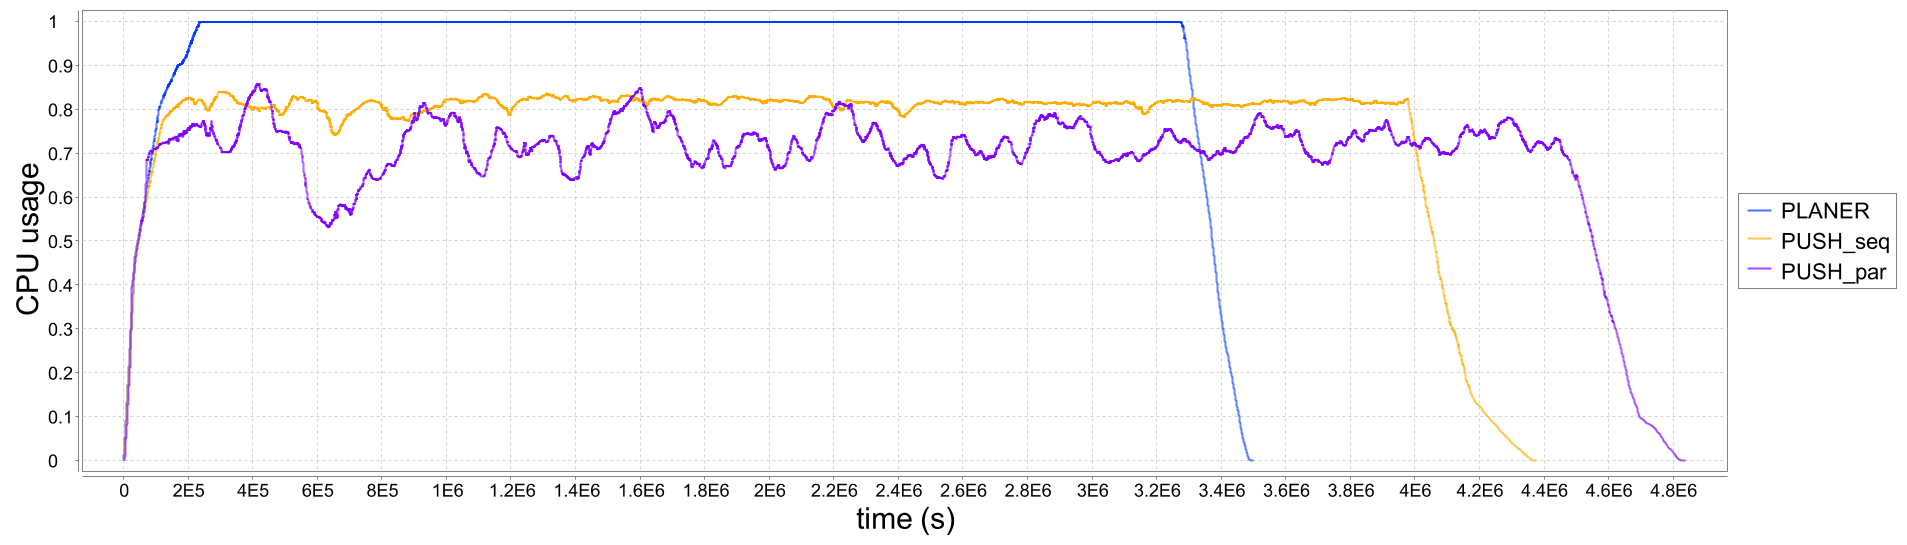
\includegraphics [trim= 0mm 00mm 0mm 00mm , clip,width=1\textwidth]{pic/3models_link01.png}
    \caption{A global CPU utilization (percentage of busy CPUs over total CPUs in the system) as a function of time for the simulation with 100 Mbps interconnecting links. The Grid structure is given at Figure \ref{simulated_grid}. A set of 60\,000 data production jobs was used for the simulations.}
      \label{multi_cpu_consumption}	
  \end{center}  
\end{figure}

After these simulations we can conclude that the proposed model can successfully utilize available network capacity including indirect links in order to "preplace" data for computations. This can lead to a significant performance improvement comparing to the traditional job distribution approaches, when data is transferred during the computation and over direct links only. 

\section{Conclusion}
\label{Conclusion}

In this paper we proposed a model of distributed data production, where all
the files from a single source has to be processed once and transferred back.
This model allows planning of WAN, storage and CPU loads using the network
flow maximization approach. The proposed model will enable automated and scalable planning and optimization of distributed computations which are highly required in data intensive computational fields such as High Energy and Nuclear Physics. Compared to the currently used data production scheduling the model provides three degrees of optimization: transferring data in advance before computation which allows to decrease IO latency; transferring  files sequentially in coordinated manner, which allows to reduce the influence of network bottlenecks; and balancing of the network traffic, which includes splitting the load between several alternative transfer paths.

The model was tested using one of the standard tools for Grid simulation (GridSim). The data extracted form the log database of real data production framework of the STAR experiment was used as input for simulations. The simulations has shown that the proposed model systematically provides better performance for distributed computations, which can reach up to 26\% improvement compared to the current scheduling approach. According to our results, the model can help to efficiently utilize more remote computational power using a limited network bandwidth. In addition to that, in our model the jobs are submitted to CPUs only after the data can be accessed efficiently by those, otherwise the CPUs remain idle and can be assigned to other computational tasks. These factors provide more flexibility when setting up a remote data production.

We continue the development of the data production planner, as the next step we plan to verify results of the simulations using data from more HENP experiments (such as ALICE at CERN) and study the effects of a background network traffic. We also plan to study the scalability of the approach, the planner performance, and the influence of the parameters, such as planing time interval, on the quality of the solution. The final goal is to integrate the developed model into the data production framework of the experiment STAR.


\begin{acknowledgements}
This work has been supported by the Czech Science Foundation
(13-20841S, P202$/$12$/$0306),  the MEYS grant CZ.1.07/2.3.00/20.0207 of the European Social Fund (ESF) in the Czech Republic: “Education for Competitiveness Operational Programme” (ECOP) and the Office of Nuclear Physics within the U.S. Department of Energy.  
\end{acknowledgements}

\bibliography{bibliography}{}
\bibliographystyle{spmpsci}

\end{document}

\end{document}
